\section{Results}
In this section we present results of runing the simulation described in the previous section. The subsections below focus on the following research questions, 

\begin{itemize}
  \item How well does the RFEA derived ion energy distribution function represents the actual energy distribution function of ions at the bounding electrode (i.e., at G$_0$)? 
  \item What is the effect of ion space charge inside the RFEA on the space potential and electric field?  
  \item What is the effect of different spacings between grids on the RFEA derived ion energy distribution function when compared to the actual one at the bounding electrode?
\end{itemize}


\subsection{Ion energy distribution profile}
Fisrt, we run the simulation at various pressures and compared the derived ion energy disribution function with the actual energy distribution as recorded in the model at G$_0$. The RFEA configuration is as follows: 2332 stack, G$_1$=C=-60~V, G$_3$=-70~V, grid transparency 100~\%. The plasma sheath potential used is AC with maximum voltage difference across the sheath of 2000~V (i.e., V$_\text{pk-pk}$), the radio-frequency 13.56~MHz, and the plasma density $10^{16}$~m$^{-3}$. The pressure settings are 0.5, 1.0, 2.0, 5.0, 7.5 and 10.0~Pa. The model is run sweeping grid G$_2$ voltage setting from 0 to 1500~V in steps of 25~V. The number of ions whose trajectory is simulated per G$_2$ voltage step is 25000. The starting time for each ion is randomized uniformly across the radio-frequency period to represent that ions may enter the sheath at any point during the RF cycle. Each ion trajectory is followed for a total time of 1~$\mu$s. 

Figure~\ref{fig:IVcurve} shows the characteristic current-voltage curve for each model RFEA scan. The vertical axis is the ion count at the collector position. The ion count drops as the pressure is increased. 

\begin{figure}[htbp]
\centering
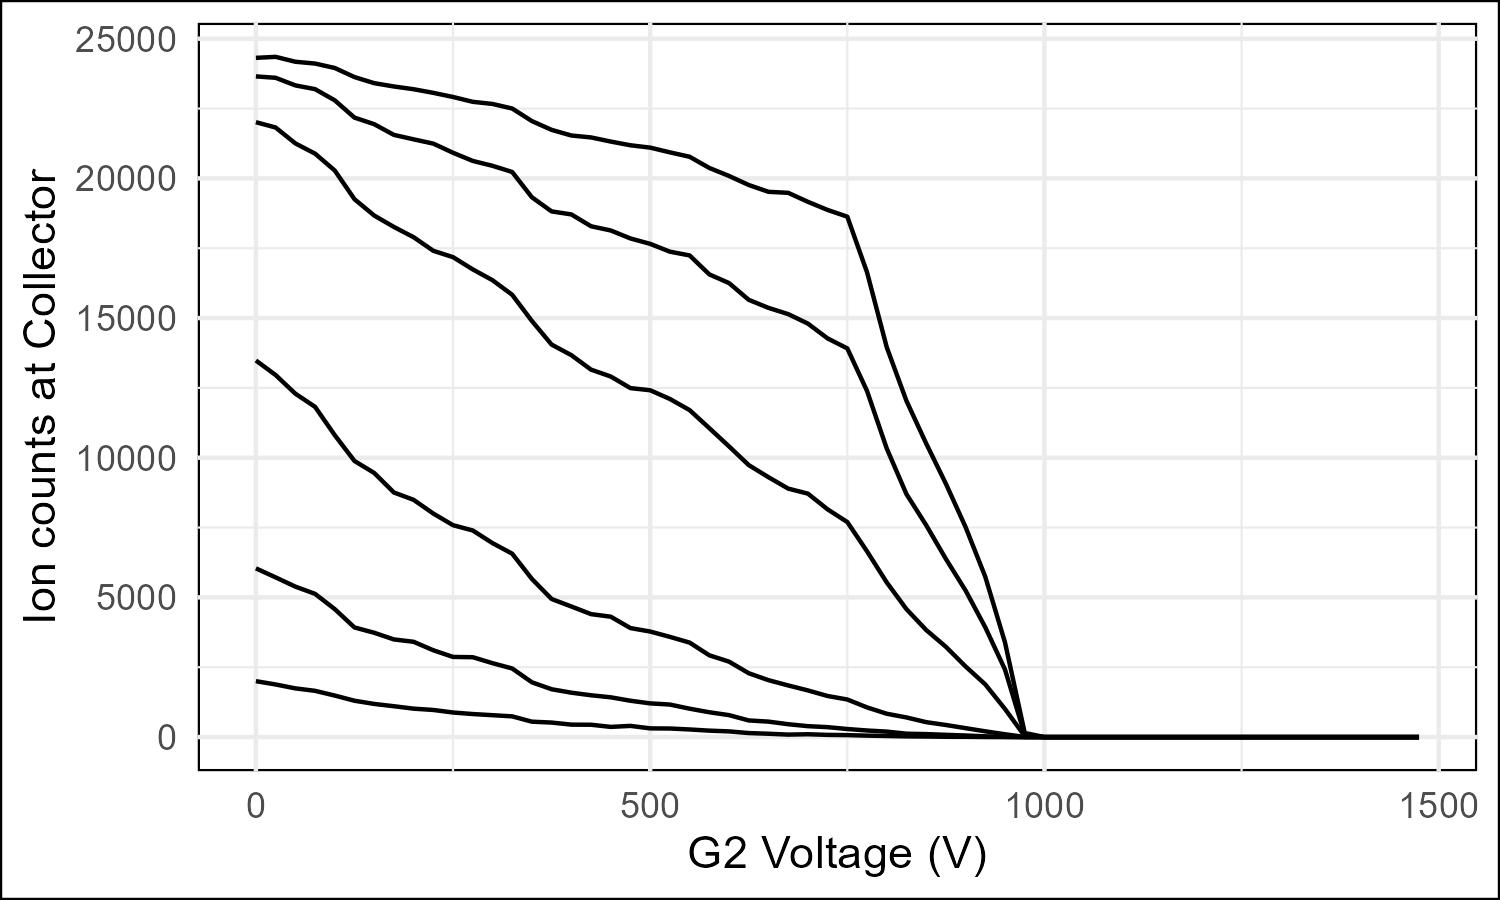
\includegraphics[width=0.45\textwidth]{Figures/IVcurve.jpeg}
\caption{Current-voltage characteristic curves where the current is represented by the ion count collected at the collector position. The curves from highest ion count value to lowest correspond to pressure settings from 0.5 to 10.0~Pa.}
\label{fig:IVcurve}
\end{figure}

The first derivative of the ion current is proportional to the ion energy distribution function~\cite{Hutchinson1987}. The set of curves on the left of Figure~\ref{fig:PressureScan} shows the first derivative of the curves in Figure~\ref{fig:IVcurve}. The derivatives are normalized and plotted with an offset in the vertical axis from lowest pressure setting at the top to highest pressure setting at the bottom. The ion energy distributions derived from the ion counts at the collector in the simulated RFEA for the various pressure settings can be contrasted with the actual ion energy distributions recorded at G$_0$, before the ions transport through the RFEA. These IEDFs are shown on the right of Figure~\ref{fig:PressureScan}. These scan were repeated with using a smaller integration time step, $dt=10$~ps, to assess any potential artifact introduced in the simulation by the trajectory integration method. No substantial qualitative difference on the energy distribution functions was observed (not shown). The derived IEDF at the collector exhibits more noise than the IEDF at G$_0$ due to the nature of the numerical derivative of the collector ion count; i.e., numerical derivatives of any parameter always ampiflies the parameter's noise. Here, a centered finite difference method was used to differentiate the Collector ion counts. All curves are shown without any smoothing.    

\begin{figure}[htbp]
\centering
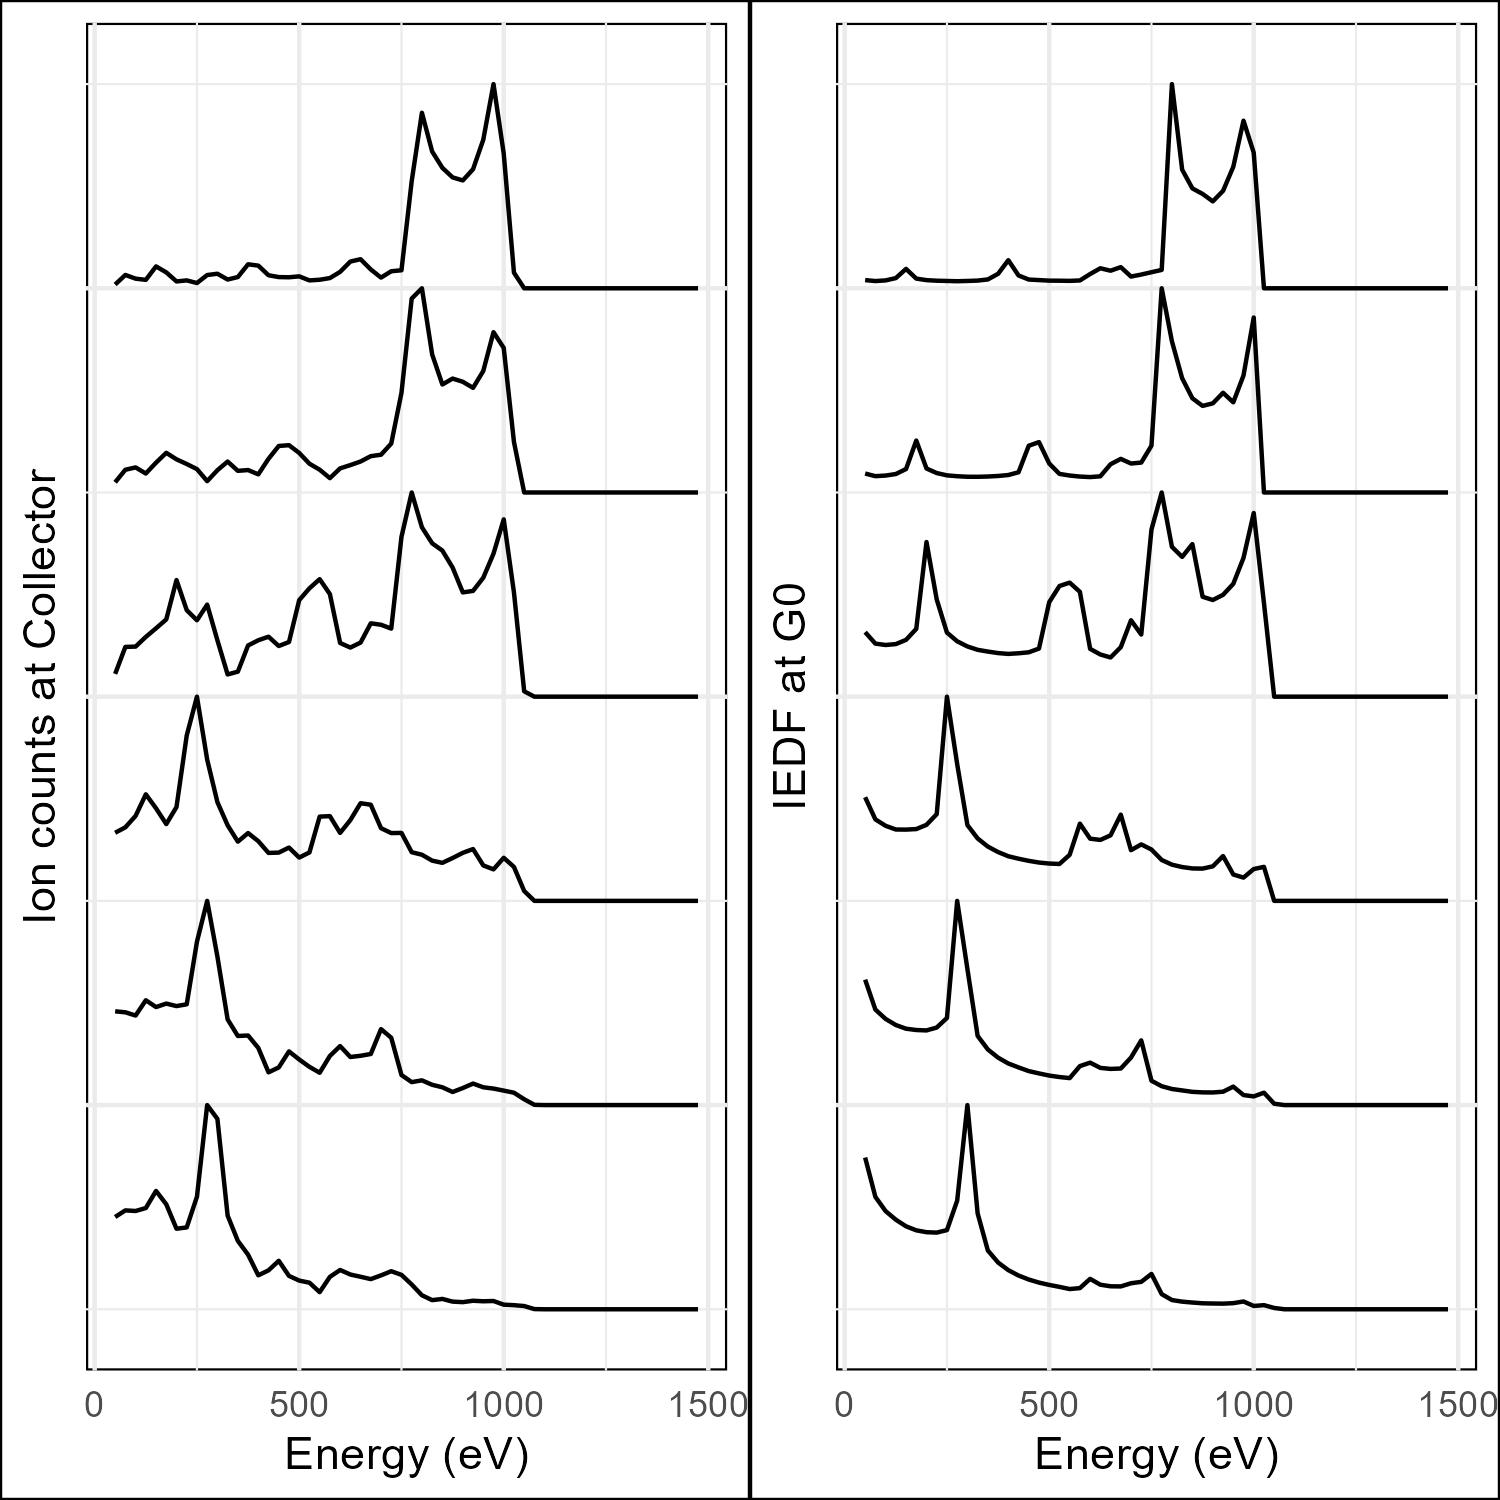
\includegraphics[width=0.45\textwidth]{Figures/PressureScan.jpeg}
\caption{Ion energy distribution functions. Left: First derivative of the current-voltage characteristic curves of Figure~\ref{fig:IVcurve}. Right: Plot of the ion energy distribution as recorded in the simulation at G$_0$, before ion transport through the RFEA. Both set of curves are normalized. The curves from top to bottom correspond to pressure settings from 0.5 to 10.0~Pa.}
\label{fig:PressureScan}
\end{figure}

The ion energy distributions of Figure~\ref{fig:PressureScan} exhibit a series of peaks which are the result of the oscillating plasma sheath and ion collisions with the background gas. More specifically, the sheath modulation, i.e., the time varying sheath edge and sheath electric field, can shape specific features of the IEDFs~\cite{Wild1989,Wild1991}. 

 